\documentclass[a4paper,11pt]{article}
\usepackage[top=2cm,bottom=2cm,left=2cm,right=2cm]{geometry}
\usepackage[utf8]{inputenc}
\usepackage[frenchb]{babel}

\usepackage{multirow}
\usepackage{makecell}
\usepackage{fancyhdr}
\usepackage{caption}
\usepackage[final]{pdfpages}
\usepackage{tikz,pgfplots,pgf}
\usepackage{subcaption}
\usepackage{siunitx}
\usepackage[toc,page]{appendix}
\usepackage{tcolorbox, listings} 
\usepackage{sectsty}
\usepackage[french]{minitoc} 
\usepackage{hyperref}
\usepackage{colortbl}
\usepackage{mwe}
\usepackage{amsmath}
\usepackage{lipsum}
\usepackage{enumitem}

\definecolor{Pantone2377C}{HTML}{2C5574}
\definecolor{subtitlecolour}{HTML}{00A2A9}
\definecolor{codegreen}{rgb}{0,0.6,0}
\definecolor{codegray}{rgb}{0.5,0.5,0.5}
\definecolor{codeblue}{HTML}{3E8BC0}
\definecolor{codeorange}{HTML}{ffa334}
\definecolor{backcolour}{HTML}{efefef}

\lstdefinestyle{myPython}{
    language=Python,
    backgroundcolor=\color{backcolour},   
    commentstyle=\color{codegreen},
    otherkeywords={plt, np, df},
    keywordstyle=\color{codeblue},
    numberstyle=\tiny\color{codegray},
    stringstyle=\color{codeorange},
    basicstyle=\ttfamily\footnotesize,
    breakatwhitespace=false,         
    breaklines=true,                 
    keepspaces=true,                 
    numbers=left,       
    numbersep=5pt,                  
    showspaces=false,                
    showstringspaces=false,
    showtabs=false,                  
    tabsize=2,
    inputencoding=utf8
}

\lstdefinestyle{myLog}{
    backgroundcolor=\color{backcolour},   
    basicstyle=\ttfamily\footnotesize,
    breakatwhitespace=false,         
    breaklines=true,                 
    keepspaces=true,                 
    numbers=left,       
    numbersep=5pt,                  
    showspaces=false,                
    showstringspaces=false,
    showtabs=false,                  
    tabsize=2,
    inputencoding=utf8
}

\lstset{
  backgroundcolor=\color{backgroundColour},   
  commentstyle=\color{codegreen},
  keywordstyle=\color{codeblue},
  numberstyle=\tiny\color{codegray},
  stringstyle=\color{codeorange},
  basicstyle=\footnotesize,
  breakatwhitespace=false,         
  breaklines=true,                 
  captionpos=b,                    
  keepspaces=true,                 
  numbers=left,                    
  numbersep=5pt,                  
  showspaces=false,                
  showstringspaces=false,
  showtabs=false,                  
  tabsize=2,
  literate=
  {é}{{\'e}}1
  {è}{{\`{e}}}1
  {ê}{{\^{e}}}1
  {û}{{\^{u}}}1
  {ù}{{\`{u}}}1
  {â}{{\^{a}}}1
  {à}{{\`{a}}}1
  {ç}{{\c{c}}}1
  {Ç}{{\c{C}}}1
  {ô}{{\^{o}}}1
}

\hypersetup{
	colorlinks=true, %colorise les liens
	breaklinks=true, %permet le retour à la ligne dans les liens trop longs
	urlcolor= blue,  %couleur des hyperliens
	linkcolor= black, %couleur des liens internes
	plainpages=false  %pour palier à "Bookmark problems can occur when you have duplicate page numbers, for example, if you have a page i and a page 1."
}

% Entête et pied de page
\pagestyle{fancy}
\rhead{
\includegraphics [scale=0.035]{img/ensta-logo.png}}
\chead{}
\lhead{}
\lfoot{Tanguy ROUDAUT - Tadios QUINIO}
\rfoot{FIPA promotion 2024}
\cfoot{\thepage}
\renewcommand{\headrulewidth}{0.4pt}
\renewcommand{\footrulewidth}{0.4pt}


\title{TP6: Inférences statistiques pour deux échantillons}
\author{Tanguy ROUDAUT — Tadios QUINIO \and FIPASE 24}
\date{18 Octobre 2022}

\begin{document}

\maketitle

\section{Bien doser l’alliage}
\vspace{.2cm}

\noindent
On teste la résistance à la traction de sept éprouvettes pour quatre aciers différents. \\

\begin{center}
    \begin{tabular}{| c | c | c | c | c | c | c | c |}
        \hline
        \multirow{2}{*}{\textbf{Proportion de carbone}} & \multicolumn{7}{ c |}{\textbf{Résistance à la traction}}\\ \cline{2-8}
                                                        & n°1 & n°2 & n°3 & n°4 & n°5 & n°6 & n°7 \\ \hline
        $0.1\%$ & 23.05 & 36 & 31.1 & 32.65 & 30.9 & 31.4 & 30.85 \\ \hline
        $0.2\%$ & 41.85 & 25.65 & 46.7 & 34.5 & 36.65 & 31.45 & 36.13 \\ \hline
        $0.4\%$ & 47.05 & 43.45 & 43 & 38.65 & 41.85 & 35.45 & 41.57 \\ \hline
        $0.6\%$ & 49.65 & 73.9 & 66.45 & 74.55 & 62.4 & 63.75 & 65.11 \\ \hline
    \end{tabular}
\end{center}
\vspace{.2cm}


\noindent
Dans un premier temps, on peut préparer le programme avec les valeurs que nous avons~:

\begin{lstlisting}[style=myPython, caption=Exploitation de l'énnoncé, frame=lines]
p = 4
n = 7

resistance_01 = [23.05, 36, 31.1, 32.65, 30.9, 31.4, 30.85]
resistance_02 = [41.85, 25.65, 46.7, 34.5, 36.65, 31.45, 36.13]
resistance_04 = [47.05, 43.45, 43, 38.65, 41.85, 35.45, 41.57]
resistance_06 = [49.65, 73.9, 66.45, 74.55, 62.4, 63.75, 65.11]
p_carbonne    = [0.1, 0.2, 0.4, 0.6]

resistance = [resistance_01, resistance_02, resistance_04, resistance_06]
\end{lstlisting}

\vspace{.5cm}
%%%%%
\begin{itemize}[label={},itemindent=-2em,leftmargin=2em]
    \item \textbf{Question~1~:} Identifier la nature des deux variables aléatoires de ce problème.
\end{itemize}
\vspace{.2cm}

\begin{itemize}
    \item Variables qualitatives ordinales $\to$ les différentes proportions de carbone
    \item Variables quantitatives discrètes $\to$ les différentes résistances
\end{itemize}


\vspace{.5cm}
%%%%%
\begin{itemize}[label={},itemindent=-2em,leftmargin=2em]
    \item \textbf{Question~2~:} Calculr les moyennes et les variances de chaque sous-population définie par la proportion
    de carbone. Représenter les boites à moustaches sur une même figure. Commenter qualitativement
    la figure résultante quant à l’influence de la proportion de carbone sur la résistance à la traction.
\end{itemize}
\vspace{.2cm}

\clearpage

\begin{itemize}
    \item \textbf{Calcul de la moyenne:}  $\overline{y}_{i\bullet}=\frac{1}{n_{i}} \sum^{n_{i}}_{j=1} y_{ij}$ \\
    \begin{lstlisting}[style=myPython, caption=Calcul de la moyenne, frame=lines]
resistance_classe_mean = []
for i in range(p):
    sum = 0
    for j in range(n):
        sum += resistance[i][j]
    resistance_classe_mean.append(sum/n)
\end{lstlisting}

    \item \textbf{Calcul de la variance:}  $S_{i}^{2}=\frac{1}{n_{i}-1} \sum^{n_{i}}_{j=1} (y_{ij}-\overline{y}_{i\bullet})$ \\
    \begin{lstlisting}[style=myPython, caption=Calcul de la variance, frame=lines]
resistance_classe_var = []
for i in range(p):
    sum = 0
    for j in range(n):
        sum += (resistance[i][j] - resistance_classe_mean[i])**2
    resistance_classe_var.append(sum/(n-1))
\end{lstlisting}

    \item \textbf{Résultat:} \\
    
    \begin{lstlisting}[style=myPython, caption=Affichage du résultat, frame=lines]
print("Question 2:")
for i in range(p):
    print("\t--> ", p_carbonne[i], "% de carbonne: moy =", resistance_classe_mean[i], " et var =", resistance_classe_var[i])
\end{lstlisting}

    \begin{lstlisting}[style=myLog, caption=Résultat, frame=lines]
Question 2:
    -->  0.1 % de carbonne: moy = 30.850  et var = 15.161
    -->  0.2 % de carbonne: moy = 36.132  et var = 46.517
    -->  0.4 % de carbonne: moy = 41.574  et var = 13.611
    -->  0.6 % de carbonne: moy = 65.115  et var = 69.396
\end{lstlisting}
    

    \item \textbf{Boite à moustaches:} \\
        \begin{figure}[!h]
            \centering
            \begin{minipage}{.48\linewidth}
                Grâce à la boite à moustache (figure~\ref{fig:figure1}) et aux valeurs précédentes, on constate facilement que la proportion de carbone à une influence sur la résistance à la traction. \\
                Si l’on prend les deux extrémités, soit une proportion de carbone de $0.1\%$ et $0.6\%$ nous obtenons les valeurs suivantes~: \\
                \begin{center}
                    \begin{tabular}{| c | c | c | c |}
                        \hline
                        \textbf{Proportion} & \textbf{min} & \textbf{max} & \textbf{moy} \\ \hline
                        $0.1\%$ & 23.05 & 36 & 30.850 \\ \hline
                        $0.6\%$ & 49.65 & 74.55 & 65.115 \\ \hline
                    \end{tabular}
                \end{center}
                \vspace{.2cm}

                Ce qui nous permet de dire que la proportion de carbone à bien une influence sur la résistance à la traction, la proportion de $0.6\%$ à une valeur max, min, quartile 1/2/3 plus important 
                que la proportion de $0.1\%$.

            \end{minipage}\hfill
            \begin{minipage}{.48\linewidth}
                \begin{center}
                    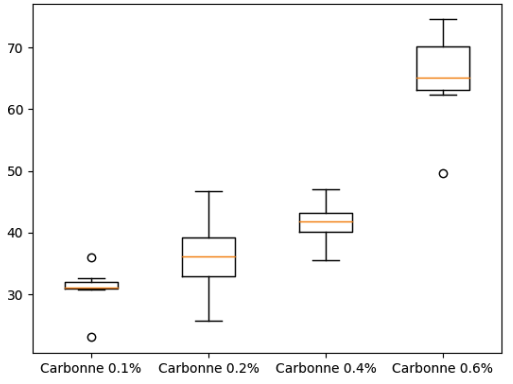
\includegraphics[width=.9\textwidth]{img/figure1.png}
                    \caption{\label{fig:figure1}Boite à moustache de la résistance à la traction de sept éprouvettes pour différent acier}
                \end{center}
            \end{minipage}
        \end{figure}
\end{itemize}


\vspace{.5cm}
%%%%%
\begin{itemize}[label={},itemindent=-2em,leftmargin=2em]
    \item \textbf{Question~3~:} Mener ce test en adoptant la procédure générale des tests. Répondre à la question: la
    proportion de carbone a-t-elle une influence sur la résistance à la traction ? On utilisera \textit{scipy.stats.f.ppf} et \textit{scipy.stats.f.cdf}
\end{itemize}
\vspace{.2cm}


\begin{itemize}
    \item \textbf{Calcul de la moyenne globale:}  $\overline{y}_{\bullet\bullet}=\frac{1}{N} \sum^{p}_{i=1} \sum^{n}_{j=1} y_{ij}$ \\
    \begin{lstlisting}[style=myPython, caption=Calcul de la moyenne globale, frame=lines]
N = p * n
resistance_global_mean = 0
for i in range(p):
    for j in range(n):
        resistance_global_mean += resistance[i][j]
resistance_global_mean /= N
\end{lstlisting}
    
    \item \textbf{Calcul de la dispersion intraclasse totale:}  $S_{W}^{2}=\frac{1}{N} \sum^{p}_{i=1} n_{i}S_{i}^{2}$ \\
    \begin{lstlisting}[style=myPython, caption=Calcul de la dispersion intraclasse totale, frame=lines]
disp_intraclasse_tot = 0
for i in range(p):
    disp_intraclasse_tot += (n*resistance_classe_var[i])
disp_intraclasse_tot /= N
\end{lstlisting}
    
    \item \textbf{Calcul de la dispersion interclasse:}  $S_{B}^{2}=\frac{1}{N} \sum^{p}_{i=1} n_{i}(\overline{y}_{i\bullet}-\overline{y}_{\bullet\bullet})^{2}$ \\
    \begin{lstlisting}[style=myPython, caption=Calcul de la dispersion interclasse, frame=lines]
disp_interclasse = 0
for i in range(p):
    disp_interclasse += n*(resistance_classe_mean[i]-resistance_global_mean)**2
disp_interclasse /= N
\end{lstlisting}

    \item \textbf{Résultat:} \\
    \begin{lstlisting}[style=myPython, caption=Affichage du résultat, frame=lines]
print("Question 3 - CALCUL:")
print("\t--> Moyenne global=", resistance_global_mean)
print("\t--> Dispersion intraclasse totale=", disp_intraclasse_tot)
print("\t--> Dispersion interclasse=", disp_interclasse, end="\n\n")
\end{lstlisting}

    \begin{lstlisting}[style=myLog, caption=Résultat, frame=lines]
Question 3 - CALCUL:
    --> Moyenne global= 43.418214285714285
    --> Dispersion intraclasse totale= 36.171686904761906
    --> Dispersion interclasse= 171.30450446428577
\end{lstlisting}

\end{itemize}

\begin{enumerate}
    \item \textbf{Grandeur d'intérêt~:} Proportion de carbone.
    \vspace{.1cm}
   \item \textbf{Hypothèse nulle, $H0$~:} La proportion de carbone n'a pas d'influence sur la résistance à la traction.
    \vspace{.1cm}
   \item \textbf{Hypothèse alternative, $H1$~:} La proportion de carbone a une influence sur la résistance à la traction.
    \vspace{.1cm}
   \item \textbf{Niveau de confiance~:} $95\%$
    \vspace{.1cm}
   \item \textbf{Test statistique~:} $F_{0} = \frac{S^{2}_{B}/(p-1)}{S^{2}_{W}/(N-p)}$ estimée par $f_{0}$ à partir de l'échantillon.
    \vspace{.1cm}
   \item \textbf{Rejet de $H0$ si~:}
        \begin{itemize}
            \item Région critique: $f_{0} > f_{\alpha, (p-1), (N-p)}$
            \item p-valeur: $p-valeur < 0.05$
        \end{itemize}

    \item \textbf{Calculs~:}
    \begin{itemize}
        \item Formules utilisées:
            \begin{figure}[!h]
                \centering
                \begin{minipage}{.48\linewidth}
                    \begin{equation}
                        f_{0} = \frac{S^{2}_{B}/(p-1)}{S^{2}_{W}/(N-p)}
                    \end{equation}
                \end{minipage}\hfill\vline
                \begin{minipage}{.48\linewidth}
                    \begin{equation}
                        f_{\alpha, (p-1), (N-p)} = F^{-1}_{F_{0}}(1 - \alpha)
                    \end{equation}
                \end{minipage}
            \end{figure}

            \begin{equation}
                \textit{p-valeur} = 1 - F_{f_{\alpha, (p-1), (N-p)}}(f_{0})
            \end{equation}    
    \end{itemize}
        \vspace{.2cm}

\begin{lstlisting}[style=myPython, caption=Code Python question 3, frame=lines]
ic = 95
alpha = 1 - (ic/100)
f = stats.f.ppf(1-alpha, (p-1), (N-p))
f0 = ((disp_interclasse)/(p-1))/((disp_intraclasse_tot)/(N-p))
p_valeur = 1 - stats.f.cdf(f0, (p-1), (N-p))

print("Question 3 - TEST:")
print("\t--> f=", f)
print("\t--> f0=", f0)
print("\t--> p-valeur=", p_valeur)
\end{lstlisting}

\begin{lstlisting}[style=myLog, caption=Résultat du code, frame=lines]
Question 3 - TEST:
    --> f= 3.0087865704473615
    --> f0= 37.88698158652568
    --> p-valeur= 2.910348628759607e-09
\end{lstlisting}


    \item \textbf{Décision~:}
        \begin{figure}[!h]
            \centering
            \begin{minipage}{.40\linewidth}
                \begin{center}
                    \begin{tabular}{| c | c |}
                        \hline
                        \multicolumn{2}{| c |}{\textbf{Critéres de rejet de H0}} \\
                        pour $\alpha$ fixé & avec \textit{p-valeur} \\ \hline
                        $f_{0} > f_{\alpha, (p-1), (N-p)}$ & $ \textit{p-valeur} < 0.05 $\\ \hline
                    \end{tabular}
                \end{center}
            \end{minipage}\hfill\vline
            \begin{minipage}{.56\linewidth}
                \begin{equation*}
                    \left .
                    \begin{aligned}
                        f_{0} = 37,886 \\
                        f_{\alpha, (p-1), (N-p)} = 3,008\\
                        \textit{p-valeur} = 2,910.10^{-09}
                    \end{aligned} \qquad
                    \right\} \qquad
                    \begin{aligned} 
                        f_{0} > f_{\alpha, (p-1), (N-p)}\\
                        \textit{p-valeur} < 0.01
                    \end{aligned}
                \end{equation*}
            \end{minipage}
        \end{figure}

        Les résultats du test statistique sont hautement significatifs, ils montrent que \textit{H0} peut être rejeté puisque toutes les conditions sont validées. \\
        La VA ne suit pas une loi de Fisher, soit la proportion de carbone a une influence sur la résistance à la traction.
\end{enumerate}


\section{Code complet}
\begin{lstlisting}[style=myPython, caption=Code Python complet TP3, frame=lines]
from scipy import stats
import numpy as np

# question 1
x = np.array([0.82, 0.87, 0.77, 0.96, 0.75, 0.83, 0.87, 0.81])
xn = np.mean(x)
ecart_type_x = np.std(x, ddof=1)
n = len(x)
ic = 95
alpha = 1 - ic / 100
t = stats.t.ppf(1 - (alpha / 2), n - 1)

I = xn - (t * ecart_type_x) / np.sqrt(n)
u = xn + (t * ecart_type_x) / np.sqrt(n)

I = round(I, 3)
u = round(u, 3)

print("Question 1:\n", "Borne inférieur:", I, "\n", "Borne supérieur:", u, end="\n\n")

# question 2
x = np.array([0.84, 0.87, 0.89, 0.73, 0.84, 0.81, 0.88, 0.85, 0.89, 0.79, 0.79, 0.90,
              0.59, 0.75, 0.67, 0.76, 0.86, 0.88, 0.70, 0.75, 0.81, 0.77, 0.83, 0.84, 
              0.71, 0.78, 0.59, 0.91, 0.74, 0.68, 0.77, 0.66, 0.80, 0.74, 1.02, 0.91,
              0.55, 0.84, 0.66, 0.77])
p = np.mean(x)
ecart_type_x = np.std(x, ddof=1)
n = len(x)
ic = 95
alpha = 1 - ic / 100
z = stats.norm.ppf(1 - (alpha / 2), loc=0, scale=1)

borne_inf = p - z * (ecart_type_x/np.sqrt(n))
borne_supp = p + z * (ecart_type_x/np.sqrt(n))

borne_inf = round(borne_inf, 3)
borne_supp = round(borne_supp, 3)

print("Question 2:\n", "Borne inférieur:", borne_inf, "\n", "Borne supérieur:", borne_supp, end="\n\n")

# question 3
n = 1000
n_dupond = 500
n_durand = 250
n_duroc = 50

def intervalle_confiance(n, x, ic ):
    p = x/n
    alpha = 1 - ic / 100
    z = stats.norm.ppf(1 - (alpha / 2), loc=0, scale=1)
    borne_inf = p - z * (np.sqrt(p*(1-p)/n))
    borne_supp = p + z * (np.sqrt(p*(1-p)/n))

    return round(borne_inf, 3), round(borne_supp, 3)

borne_inf_dupond_95, borne_supp_dupond_95 = intervalle_confiance(n, n_dupond, 95)
borne_inf_durand_95, borne_supp_durand_95 = intervalle_confiance(n, n_durand, 95)
borne_inf_duroc_95, borne_supp_duroc_95 = intervalle_confiance(n, n_duroc, 95)
borne_inf_dupond_99, borne_supp_dupond_99 = intervalle_confiance(n, n_dupond, 99)
borne_inf_durand_99, borne_supp_durand_99 = intervalle_confiance(n, n_durand, 99)
borne_inf_duroc_99, borne_supp_duroc_99 = intervalle_confiance(n, n_duroc, 99)

print("Question 3:")
print(" Dupond")
print("\t --> Borne inférieur à 95%:", borne_inf_dupond_95)
print("\t --> Borne supérieur à 95%:", borne_supp_dupond_95)
print("\t\t\t ------------------------")
print("\t --> Borne inférieur à 99%:", borne_inf_dupond_99)
print("\t --> Borne supérieur à 99%:", borne_supp_dupond_99)
print(" Durand")
print("\t --> Borne inférieur à 95%:", borne_inf_durand_95)
print("\t --> Borne supérieur à 95%:", borne_supp_durand_95)
print("\t\t\t ------------------------")
print("\t --> Borne inférieur à 99%:", borne_inf_durand_99)
print("\t --> Borne supérieur à 99%:", borne_supp_durand_99)
print(" Duroc")
print("\t --> Borne inférieur à 95%:", borne_inf_duroc_95)
print("\t --> Borne supérieur à 95%:", borne_supp_duroc_95)
print("\t\t\t ------------------------")
print("\t --> Borne inférieur à 99%:", borne_inf_duroc_99)
print("\t --> Borne supérieur à 99%:", borne_supp_duroc_99, end="\n\n")

# question 4
ic = 95
alpha = 1 - ic / 100
p = 17/100
err = 1/100
z = stats.norm.ppf(1 - (alpha / 2), loc=0, scale=1)
n = (z/err)**2 * p*(1-p)
n = np.ceil(n)

print("Question 4:\n", "Nombre de personne à intérroger:", n, end='\n\n')

# question 5
n_casques = 50
n_dommages = 18
borne_inf_dommages_95, borne_supp_dommages_95 = intervalle_confiance(n_casques, n_dommages, 95)

print("Question 5:")
print(" Casques endommagés")
print("\t --> Borne inférieur à 95%:", borne_inf_dommages_95)
print("\t --> Borne supérieur à 95%:", borne_supp_dommages_95, end="\n\n")

# question 6
ic = 95
alpha = 1 - ic / 100
p = 18/50
err = .02
z = stats.norm.ppf(1 - (alpha / 2), loc=0, scale=1)
n = (z/err)**2 * p*(1-p)
n = np.ceil(n)

print("Question 6:\n", "Nombre de casque à tester:", n, end='\n\n')

# question 7
ic = 95
alpha = 1 - ic / 100
err = .02
z = stats.norm.ppf(1 - (alpha / 2), loc=0, scale=1)
p = np.linspace(0, 1, 101)
n = (z/err)**2 * p*(1-p)
index_n_max = np.where(n == max(n))
n = np.ceil(float(n[index_n_max]))

print("Question 7:\n", "Nombre de casque à tester:", n, end='\n\n')    
\end{lstlisting}



\end{document}